\documentclass[modern]{aastex61}

%% AASTeX v6.* now includes \hyperref support. While we have built in specific
%% defaults into the classfile you can manually override them with the
%% \hypersetup command. For example,
%%
%% \hypersetup{linkcolor=red,citecolor=green,filecolor=cyan,urlcolor=magenta}
\usepackage[]{graphicx}
\newcommand{\vdag}{(v)^\dagger}
\newcommand\aastex{AAS\TeX}
\newcommand\latex{La\TeX}
\newcommand{\red}[1]{\textcolor{red}{#1}}
\usepackage{ulem}

% \received{}
% \revised{}
% \accepted{}

% \submitjournal{ApJ}


\shorttitle{Gravitational Wave Counterparts Observed by TESS}
\shortauthors{Barclay et al.}

\begin{document}

\title{On the Feasibility of Using Transiting Exoplanet Survey Satellite to Observe Electromagnetic Counterparts to Gravitational Wave Events}

\correspondingauthor{Thomas Barclay}
\email{thomas.barclay@nasa.gov}

\author[0000-0001-7139-2724]{Thomas Barclay}
\affiliation{NASA Goddard Space Flight Center, 8800 Greenbelt Rd, Greenbelt, MD 20771}
\affiliation{University of Maryland, Baltimore County, 1000 Hilltop Cir, Baltimore, MD 21250}

\author{Judith L. Racusin}
\affiliation{NASA Goddard Space Flight Center, 8800 Greenbelt Rd, Greenbelt, MD 20771}

\author{Joshua E. Schlieder}
\affiliation{NASA Goddard Space Flight Center, 8800 Greenbelt Rd, Greenbelt, MD 20771}

\author{Daniel Kocevski}
\affiliation{NASA Marshall Space Flight Center, Huntsville, AL 35812}

% for now, Regina is not an author. because she's the worst
% \author{Regina M. Caputo}
% \affiliation{NASA Goddard Space Flight Center, 8800 Greenbelt Rd, Greenbelt, MD 20771}
% \affiliation{University of Maryland, College Park, MD 20742}

\author{Geert Barentsen}
\affiliation{NASA Ames Research Center, Moffett Field, CA 94035}
\affiliation{Bay Area Environmental Research Inst., 625 2nd St. Ste 209 Petaluma, CA 94952}

\author{S. Bradley Cenko}
\affiliation{NASA Goddard Space Flight Center, 8800 Greenbelt Rd, Greenbelt, MD 20771}

\author{Patricia T. Boyd}
\affiliation{NASA Goddard Space Flight Center, 8800 Greenbelt Rd, Greenbelt, MD 20771}

\author[0000-0003-1309-2904]{Elisa V. Quintana}
\affiliation{NASA Goddard Space Flight Center, 8800 Greenbelt Rd, Greenbelt, MD 20771}

\begin{abstract}

The recent detection of a kilonova associated with a neutron star merger event that produced both a gravitational wave signal and a short gamma-ray burst heralds a new era of multimessenger astrophysics. Ground and spaced based observations revealed that the kilonova emission peaked at optical wavelengths, however, detailed interpretation of this event was challenging because of a $\sim$12 hour time lag between the LIGO/Virgo and Fermi-GBM alerts and the detection of an optical counterpart. The Transiting Exoplanet Survey Satellite (TESS) will launch in 2018 and is equipped with four 24$^{\circ}$$\times$24$^{\circ}$ field-of-view cameras with a wide bandpass covering 0.6--1.0 $\mu$m. The four cameras are angled to target a contiguous 96$^{\circ}$$\times$24$^{\circ}$ field in an anti-solar direction continuously for 27 days. TESS can provide prompt optical coverage of kilonova emission by through serendipitous monitoring a single sky position. Herein, we (perhaps foolishly) extrapolate from the single known kilonova to estimate a frequency in the local Universe and use this to predict an event detection rate for TESS. Using a model that includes both on and off-axis events representing kilonovae {\textit {and}} afterglows from short-duration gamma-ray bursts with a range of potential luminosities, we predict that TESS will detect 40--530 events per century. Not all optical detections will have a GW counterpart. Accounting for the LIGO/Virgo observing windows and sensitivity, we predict $0.7^{+1.4}_{-0.5}$ joint TESS-GW events during the 2-year primary mission.
%Fortunately, TESS has the potential to run for decades in an extended mission phase; in a 10 year mission we optimistically predict that TESS could detect light from 3 kilonovae.


%We find that in the 2-year primary mission XX events will fall into the field-of-view of TESS. However, significant fractions of sky are not amenable to faint-source astrophysics from TESS because of a combination of the direct and scattered moonlight, zodiacal light and high stellar density region. 
%Therefore, TESS will detect XX events in 2-years, although with a potential 10+ year extended mission the number could be dramatically larger.

\end{abstract}

\keywords{gamma-ray burst: general, gravitational waves, stars: neutron, surveys}

\section{Introduction} \label{sec:intro}
On August 17, 2017 the Laser Interferometer Gravitational-Wave Observatory (LIGO) and Virgo observatory made the first detection of gravitational waves produced by the merger of two neutron stars.  GW170817 was followed by an unambiguous electromagnetic (EM) counterpart, GRB170817A/SSS17a/AT2017gfo, by more than 70 space and ground-based observatories \citep{Abbott2017a,Abbott2017b,Abbott2017c}. Through these combined efforts we have access to a vast array of data from this event, which can be used to make predictions for future missions and instruments. Observations cover the full electromagnetic spectrum from gamma-ray to radio \citep{Goldstein2017,Savchenko2017,Troja2017,Evans2017,Coulter2017,Kim2017,Hallinan2017}, and detection of a counterpart from 1.7 seconds to months post-merger \citep{Abbott2017b,Ruan2017}. The source of the emission was most likely a binary neutron star (BNS) merger \citep{Abbott2017a} and resulted in prompt gamma-ray emission detected by the {\it Fermi} Gamma-ray Burst Monitor (GBM) \citep{Goldstein2017} and the INTEGRAL Spectrometer Anticoincidence shield (SPI-ACS) \citep{Savchenko2017}. UV, optical, and IR observations commenced within hours, with many telescopes tiling the GBM localization region, nearby galaxies, and later the LIGO/Virgo localization region, resulting in the detection of the optical counterpart $\sim$11 hours after the GW/gamma-ray detection \citep{Abbott2017c}. The Swope telescope found a relatively bright (V$\sim$17), blue source (SSS17a/AT2017gfo) in the direction of Galaxy NGC 4993 \citep{Coulter2017}. This source, known as a kilonova or macronova, is interpreted as isotropic emission driven by the radioactive decay of rapid neutron capture process elements and showed strong spectral evolution from blue to red over the next week \citep{Villar2017}.

NGC 4993 is at a distance of $41.0\pm3.1$ Mpc \citep{Hjorth2017}, consistent with the distance constraint by LIGO/Virgo of $43.8^{+2.9}_{-6.9}$ Mpc \citep{Abbott2017d}, or z$\sim$0.01.  This is an order of magnitude closer than all previous short GRBs with measured redshifts. Short duration GRB redshifts are particularly difficult to obtain because they require either a bright well-localized optical counterpart, or firm association of a host galaxy from the X-ray, optical, or radio position.  A normal not-so-well localized GRB like GRB170817A would likely not have been followed-up by anyone, had it not been for the GW detection \citep{Goldstein2017}.

The highly-anticipated, though perhaps not quite this soon, discovery of a BNS merger in association with not only a GRB, but a kilonova is a momentous time in astrophysics. With these observations, not only do we confirm the origin of at least some short duration gamma-ray bursts, we also have the best constraints on the speed of gravity ever obtained, new understanding of the neutron star equation of state \citep{Abbott2017c}, and proof of the origin of a significant portion of r-process elements in the Universe \citep{Chornock2017,Drout2017,Pian2017,Tanvir2017}.

The spectrum of the UV/optical/IR counterpart evolved rapidly from blue to red over the first few days after the merger with a relatively featureless spectrum that cannot be simply described with a blackbody \citep{McCully2017}. The event was mostly likely observed off axis \citep{Troja2017,Abbott2017a}, but there is debate over the line-of-sight angle, with estimates ranging from 18--55 degrees \citep{Mandel2017,Abbott2017a,Kim2017,Haggard2017}.
Studies of the kilonova spectral evolution evoke explanations such as different spatial distributions and opacities of the lanthanides and actinides \citep{McCully2017,Cowperthwaite2017}, cocoon emission of a choked jet \citep{Kasliwal2017}, and wind-driven outflow \citep{Evans2017}. 
% \red{JLR: I'm surely missing some of these, anyone feel free to add.}

% \red{Some nice words from Judy that we can write around, crossing out those done:}
% \begin{itemize}
% \item \sout{spectral evolution of the kilonova - there was strong spectral evolution from blue to red over days after the event.  I saw a nice graphic during the second press panel, which was from VLT/X-shooter. }
% \item mass - there is a maximum mass of NS, which isn’t well known, but is likely not that much higher than the final mass of this system.  It’s not clear if after the merger a stable NS was formed or a BH, but there’s some evidence (late X-ray) of a BH.  I’m not sure how luminosity scales with ejecta mass.
% \item \sout{distance - This object was crazy close (z~0.01).  Most short GRBs are further away, though there are a lot of observational biases.  If one assumes that GRB170817A was on-axis, the rates of low-luminosity BNS mergers are really high.  If it was off-axis, even a little, the rates are lower.  The kilonova is isotropic, but inferences from the GRB are tricky.  Though I think the LIGO/Virgo rates might be based on GW alone.}
% \item transients - This event was also super bright because it was nearby, it might be harder to find distinctly and differentiate from other kinds of transients (especially with only one filter) if they’re further away.  How far away could TESS have detected this event at 1 hour, 12 hours, 1 day, etc.?
% \item rates - Even without a GW trigger, it would be interesting to search for ‘orphan’ kilonovae \& GRB afterglows.  The 30 minute cadence of a huge swath of the sky would be great for this.  Though what is the limiting magnitude?  What is the wavelength coverage?  It’s a statistics game since TESS won’t be following up, but rather taking serendipitous observations. 
% \item latency - Given the latency in downlinking data, it can’t really be argued strongly that TESS will inform follow-up observations.  Of course, we could get lucky, and have a downlink 1 day after a GW trigger, but it’s a statistics game.  I think TESS as an instrument to characterize a population of these events is more compelling. 
% \end{itemize}
% ...\\
% todo - define what GW range means

% todo - change opening angle to Fong et al. 2017

% ...\\
% ...\\
The Transiting Exoplanet Survey Satellite (TESS) was selected as an NASA Astrophysics Explorer-class mission in 2013 and is rapidly approaching launch, which is scheduled for the first half of 2018. The aim of the TESS mission is to identify transiting exoplanets around nearby bright stars that can be followed-up with precision radial velocity observations \citep{Ricker2015}. To accomplish this goal, TESS has four 24$^{\circ}$$\times$24$^{\circ}$ field-of-view (FOV) cameras that, as shown in Figure~\ref{fig:cameras}, target adjacent regions of the sky to make-up a single 96$^{\circ}$$\times$24$^{\circ}$ sector. The optical assemblies and detectors in each camera are identical and obtain images in a single bandpass spanning $\sim$0.6--1.0 $\mu$m. The spacecraft will be flown on an elliptical, high earth orbit with an orbital period of 13.7 days in a 2:1 resonance with the Moon. The orbital attitude is anti-solar and places the ecliptic pole at the center of the Camera 4, where cameras are numbered 1--4 from lowest to highest ecliptic latitude. Every 27.4 days (2 orbits) the spacecraft pointing will be rotated about the ecliptic pole by approximately 28$^{\circ}$ in ecliptic longitude. This observing mode allows TESS to survey nearly an entire ecliptic hemisphere in 13 adjacent sectors over a period of one year. The mission will begin by observing the southern ecliptic hemisphere; the spacecraft will then reorient to observe the northern ecliptic hemisphere in its second year. During the 2-year primary mission phase, TESS will monitor more than 200,000 preselected stars at 2-min cadence using pixel sub-apertures to accomplish its core science requirement of transiting exoplanet discovery \citep{Sullivan2015}. In addition, TESS will observe $\sim$90\% of the sky in Full-Frame Image (FFI) mode which continually takes 30-min integrations of the full 96$^{\circ}$$\times$24$^{\circ}$ FOV. 

\begin{figure}
\centering
\includegraphics[width=0.5\textwidth]{tess_cameraFOVschematic_Winnpresentation.png}
\caption{TESS has four identical cameras that combine to observe 96$^{\circ}$$\times$24$^{\circ}$ simultaneously. The cameras are numbered 1--4 in order of increasing distance from the ecliptic plane. After each 27.4 day long observing sector, TESS will rotate by approximately 28$^{\circ}$ about the center of Camera 4, to maintain an anti-solar pointing. This observing mode allows TESS will observe 13 sectors over a year; completing a survey of one ecliptic hemisphere. During its 2-year primary mission, TESS will survey $\sim$90\% of the sky with a cadence of 30-min.
\textbf{TB to make his own version of this.}}
\label{fig:cameras}
\end{figure}

The FFI data mode significantly enhances the range of science that is accessible to TESS. This is because, unlike with the 2-min cadence data, the targets do not need to be preselected. In addition to the observation of enormous numbers of relatively common targets \citep[e.g.][]{Thomas2016,Raddi2017}, the wide-FOV of the FFI mode enables the detection of transient phenomena such as stellar super-flares, novae, supernovae, tidal disruption events, and optical counterparts to gamma-ray bursts (GRBs). While the 10-cm aperture of each of the four cameras and large 21x21 arcsec pixels generally limit science to relatively bright events, the 27 day continuous stare means that integrations can be binned together over hours-to-days \citep[e.g.][]{Pal2015}. 

A challenge in interpreting transient events is that prompt optical observations are not usually not available. While the LIGO/Virgo gravitational waves and associated high-energy alerts were released within seconds of the GW170817 merger event, identification of the optical counterpart didn't happen until 11 hours later. TESS' wide FOV has the advantage of enabling serendipitous detection and monitoring of optical counterparts to these transient sources without re-pointing. Through early observations of these we can monitor the physical processes occurring at early times which will allow us to constrain emission models and catch additional components \citep[e.g.][]{Racusin2008}.  %Although TESS communications delays of days \red{[right?]} from the normal downlink schedule would likely not be able to provide prompt localization or characterization of these transients to follow-up observers, TESS will naturally follow the evolution at regular uninterupted 30 minute cadence over a very large swath of the sky.  
If TESS were already flying when GW170817 occurred, and it happened to be in the TESS FOV, optical observations would cover the neutron star merger, avoiding the 11 hour delay spent hunting for a counterpart. %from {\it Fermi}-GBM localization (seconds after trigger) and the LIGO/Virgo localization ($\sim$5 hours).

Kepler observations of supernovae \citep{Olling2015,Garnavich2016} have demonstrated the compelling science associated with rapidly getting on source. Neither Kepler nor TESS are especially useful for triggering other observations because they do not continually downlink data, but rather they can serendipitously observe the rise and fall of transient phenomena. TESS has a number of advantages over Kepler in this area. The TESS field of view is roughly 20 times larger than Kepler, TESS downloads the entire field at 30 min cadence rather than $\lesssim$5\% of pixels for Kepler, and the data are downlinked to the ground more frequently -- every 13.7 days vs. 30--90 days. Kepler though, has a much larger collecting area (Kepler has a 1m aperture vs. 10cm for TESS), meaning it can go about 5 magnitudes fainter. Kepler also has a bluer bandpass, which for GW170817 would have resulted in a higher flux. Nevertheless, with TESS beginning science operation in mid-2018 and LIGO/Virgo continuing to increase in sensitivity for the O3 observing run ($\sim$ late-2018 or 2019), there is potential for high value, multi-messenger science from joint detections. The aim to this study is to determine whether TESS can contribute to the coming decade of GW+EM science. 

\section{Calculating the yield}
\subsection{The brightness of GW170817 in the TESS bandpass}
% The first step we need to perform is to create a population of EM counterparts. We can then assess whether we could detect these events from TESS. Initially, we make a simplistic assumption: all future events will look exactly like GW170817. 
The first step we will take is to simulate what TESS would have observed for GW170817. \citet{Shappee2017} presented a series of 8 optical spectra taken from using the LDSS-3, MagE, and IMACS spectrographs on the Magellan telescopes at times after the LIGO/Virgo detection of T$_0$ + [0.49, 0.53, 1.46, 2.49, 3.46, 4.51, 7.45, 8.46] days. We took these spectra and convolved them with the quantum efficiency of the TESS bandpass \citep{Ricker2015}, the resulting bandpass-convolved spectra are shown in Figure~\ref{fig:spectra}. First two spectra peak in the blue, outside the TESS bandpass at around 0.4$\mu$m. Over time the spectra get redder and fainter.

\begin{figure}
\centering
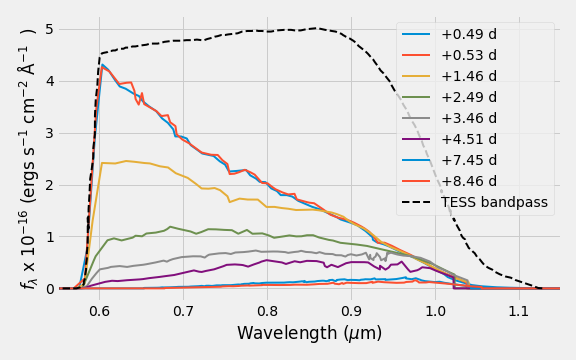
\includegraphics[width=0.8\textwidth]{tess-convolved-spectra-gw20170817.png}
\caption{Optical spectra of GW170817 convolved with the TESS bandpass. The spectra are taken using various instruments on the Magellan telescopes and cover a time from 0.49--8.46 days post-merger \citep{Shappee2017}. The early spectra peak in the blue, outside the TESS bandpass, and get redder and fainter over time.}
\label{fig:spectra}
\end{figure}
We then calculated an AB magnitude \citep{Oke1983} in the TESS bandpass for each spectrum by converting the fluxes to spectral densities per unit frequency, and then integrating over both the bandwidth-convolved spectra and the bandwidth to calculate
\begin{equation}
m_{AB} = -2.5\log{ \left(\frac{\int{f_\nu\, \mathrm{QE}_\nu\, \mathrm{d}\nu}}{\int{3631 \mathrm{Jy}\,  \mathrm{QE}_\nu\, \mathrm{d}\nu}} \right )}
\end{equation}
following Equation 4 of \citet{Tonry2012}, where $\mathrm{QE}_\nu$ is the bandpass quantum efficiency, and $m_{AB}$ is the calculated magnitude. 

The Magellan spectra average at one per day over eight days. However, TESS will readout every 30-min. To simulate TESS data we interpolated between T$_0$+0.49 and 8.46 days, and extrapolated to times earlier than T$_0$+0.49 days using a cubic spline and evaluated the resulting function at 30-min intervals. For each of the 30-min data-points we calculated the TESS 1-$\sigma$ 1-hr integrated noise level following \citet{Ricker2015} and multiplied by $\sqrt{0.5}$ to account for decreased exposure time\footnote{We caution against using the TESS photometric precision level presented by \citet{Stassun2017} for faint sources because they are unreliable at magnitudes greater than 16}. 

Due to TESS's 21$\times$21 arcsecond pixels, most galaxies will not be resolved from the kilonova. This adds an additional noise term which is the Poisson error in counts associated with the galaxy. Following \citet{Bouma2017}, the TESS count-rate scales with the brightness of the galaxy as
\begin{equation}
\mu = 1.514\times10^6 \times 69.1 \times 3600 \times 10^{- \frac{m}{2.5}}
\end{equation}
where 69.1 cm$^2$ is the collecting area of the telescope, 3600 s is a 1-hour integration, and $m$ is the brightness of the source in TESS-bandpass magnitudes. The Poisson noise from the Galaxy counts is $\sigma_G\approx\mu^{1/2}$. We took the model spectrum of NGC 4993 presented by \citet{Troja2017} and convolved and integrated over the TESS bandpass to derive a Tmag brightness of 11.3 for NGC 4993. The integrated surface brightness of NGC4993 approximately 6 magnitudes (250x) brighter than for the kilonova. These extra count equate to an additional 7.4\% uncertainty added in quadrature for a 1-hour integration, or 10\% for a 30-min integration at peak kilonova brightness. 

In Figure~\ref{fig:tesslc} we show a simulated TESS light curve of GW170817, a peak brightness of Tmag=17.3 occurs at $T_0$+0.7 days. This is in good agreement with times series data presented by \cite{Arcavi2017}. The scatter on the data shown in the figure is a single draw from a multivariate normal distribution, with standard deviation calculated from the uncertainty. The host galaxy has been subtracted but the additional uncertainty from the host galaxy flux is included. This event observed by TESS would have been above a 5-$\sigma$ per detection 30-min integration while above Tmag=18.12, which is the first 2.6 after the merger. The uncertainty exceeds half a magnitude once the target is fainter than Tmag=18.2, which occurs at T$_0$+2.9 days. If we relax our time resolution needs, we can integrate over several hours to build up counts. In a 6-hours integration we can make a 5-$\sigma$ detection while the target is brighter than Tmag=18.4, which occurs at T$_0$+3.3 days.

\begin{figure}
\centering
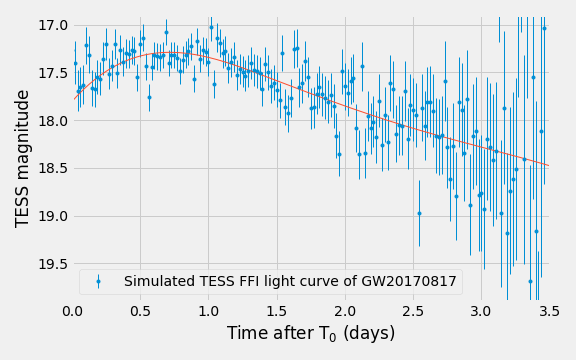
\includegraphics[width=0.8\textwidth]{tess-lc-gw20170817-v3.png}
\caption{Simulated TESS light curve of GW170817. The 30-min integrations have realistic noise properties and includes the additional light from the host galaxy. This demonstrate the ability of TESS to perform relatively precise photometry in the first few days after a BNS merger. After the targets get below a Tmag of 18.2 the photometry becomes poor.}
\label{fig:tesslc}
\end{figure}

\begin{figure}
\centering
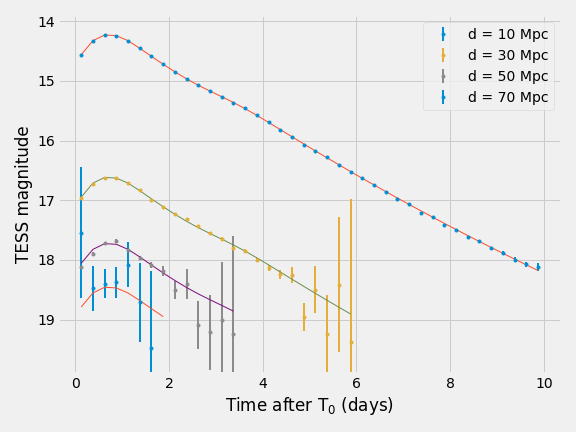
\includegraphics[width=0.8\textwidth]{tess-lc-various-distances.png}
\caption{Simulated TESS light curves of kilonovae a various distances. The data plotted show are 6-hour integrations and data points are only plotted if the uncertainty is $<$100\%. High quality data of the first 2 days post-merger can be collected out to 50--60 Mpc. Beyond this, features in the light curve become difficult to disentangle from noise.}
\label{fig:tesslc-distances}
\end{figure}


\subsection{Simulating the EM counterpart population}
% GW170817 occurred in the galaxy NGC 4993 which is $41\pm3$ Gpc away from us \citep{}. We used this luminosity distance to convert from apparent to absolute magnitude and found a peak absolute TESS magnitude of -15.8. Additionally, this implies an absolute Tmag of the host galaxy, NGC 4993, of Tmag=-21. 
%
To simulate the population we need need to estimate several things: the range in brightness of host galaxies, the range of brightness of optical counterparts to GW events, and the frequency and distance of events. While there is a dispersion in the absolute magnitudes of galaxies the distribution of $i$-band absolute magnitude of galaxies is $-20.9\pm1.0$ \citep{Blanton2003}., making NGC 4993 at Tmag=-21 typical.

For the frequency of events we need to assume an occurrence rates for BNS merger events. \citet{Abbott2017a} estimate $1540^{+3200}_{-1220}$ Gpc$^{-3}$ yr$^{-1}$, which we adopt here. 

GW170817 was most likely observed off-axis. However, a subset of future events will be observed on-axis where we can observe both the kilonova and a GRB optical afterglow. \citet{Metzger2012} show models that predict that these on-axis bursts with an associated afterglow could be 3--130 more energetic at peak brightnesses than GW170817. The range of opening angles is relatively poorly constrained but is estimated to be around 16$^\circ$ \citep{Fong2015}, which means that approximately 3.9\% of observed events will be observed on-axis. 
Furthermore, \citet{Metzger2012} show a range of peak brightnesses for off-axis events, such as GW170817, range from 0.3--13 times as bright as the event we observed. 

We assume that 3.9\% of events range in brightness between 3--130x the peak brightness GW170817, and the remaining events are 0.3--12x the brightness of GW170817. We assume that this is distributed log-uniformly. Assuming that the location of BNS mergers is distributed isotropically, we simulated 100 years of events in a sphere of volume 10 Gpc$^3$, with Earth at the center. We can than determine which of these events would be detected, assuming a detection is something that measured above 5-$\sigma$ in a 6-hour integration. This amounts to 2400$^{+5000}_{-1900}$ on-axis GRB afterglows and 1900$^{+3700}_{-1500}$ kilonovae per century detectable by TESS. However, TESS is not observing the whole sky simultaneously.



% Using Tmag=18.4 as our faint limit results in a sensitivity mergers occurring with 67 Mpc. We predict that $180^{+430}_{-150}$ events \red{with the properties of GW170817,} \sout{that} are bright enough to be detectable by TESS \sout{will occur} per century. However, TESS does not observe all the sky and is not observing all the time. 

TESS has an instantaneous field of view of 96x24 degrees, 5.6\% of the sky, but the telescope does not observe continuously. There are breaks of around 16 hours every 13.7 days when the spacecraft reorientates to point the high-gain Ka-band antenna toward Earth, enabling high-bandwidth data downlinks. For simplicity, we will assume that 95\% of detections in the TESS field of view are obtained and 5\% are missed. We are ignoring where the event peak is missed. In addition to the breaks in observations, not all the sky is suitable for the detection of faint stars with TESS. The large pixels of TESS (21x21 arcsec) mean that regions close to the Galactic plane are inaccessible. For simplicity we assume that no events are detectable closer than $\pm$10 deg from the Galactic plane, this rules out 16.1\% of the TESS field of view. Furthermore, the Moon and Earth will regularly pass through the TESS field of view ruling out a further 8.7\% of the TESS field of view \citep{Bouma2017}. Therefore, our final effective instantaneous sky coverage is 4.1\% of the celestial sphere.

Multiplying the all-sky rates by 4.1\% yields a rate per century detected by TESS of 95$^{+210}_{-75}$ for on-axis and 75$^{+160}_{-60}$ for off-axis. The distances of these simulated events range from  170--720 Mpc for on-axis, and 55--230 Mpc for off-axis.

% We simply multiply the number of detectable events by the TESS instantaneous sky coverage to give our predicted number of BNS merger events detected by TESS: $180^{+430}_{-150} \times 0.041=8^{+18}_{-6}$ per century. In the nominal primary mission of 2-years we predict TESS will be quite unlikely to detect any events.

% \subsection{Line-of-sight and other effects}
% We made a number of simplistic assumptions in the previous section, but the most unreasonable one is that future kilonova will look exactly like GW170817. This is, of course, not very likely. GW170817 was most likely observed off-axis \citep{Troja2017,Abbott2017a}. However, a subset of future events will be observed on-axis. \citet{Metzger2012} show models that predict that these on-axis bursts could be 3--130 more energetic at peak brightnesses than GW170817. 
% %Typical opening angles are in the region of 7 degrees \citep{Soderberg2006,Burrows2006}, which means that approximately 0.75\% of observed events will be observed on-axis. 
% The range of opening angles is relatively poorly constrained but is estimated to be around 16$^\circ$ \citep{Fong2015}, which means that approximately 3.9\% of observed events will be observed on-axis. 
% Furthermore, \citet{Metzger2012} show a range of peak brightnesses for off-axis events such as GW170817 range from 0.3--13 times as bright as the event we observed. \red{JLR: This is a bit confusing because the kilonova is isotropic, what is seen on-axis is the GRB afterglow.}

% We performed the same simulations described above but this time modified the absolute magnitude of each merger event by adding a constant brightness modifier. The constant is drawn from a log-uniform distribution in flux. For 3.9\% of events the flux offset is between 3--130x the peak brightness GW170817, and for the remaining events 0.3--12x the brightness of GW170817. \red{JLR: we have some handle on the spectra of on-axis afterglow with power law spectra with photon indicies ~1.5-3 (Fong et al. 2015).  Also, are you accounting for dust in both our galaxy and the host?}

% This has a fairly dramatic effect. The number of observed events increases by almost an order of magnitude -- from $8^{+18}_{-6}$ to $87^{+360}_{-69}$ per century. Of these, $15^{+29}_{-11}$ ($17$\%) come from on-axis and $72^{+160}_{-59}$ ($83$\%) from off-axis events. 

% Without including the variable brightness we were only sensitive to BNS mergers out to 67 Mpc (where the peak brightness has Tmag$<$18.4). With this more complex model, we find 90th percentile distances of detected events at 140--610 Mpc for on-axis and 48--220 Mpc for off-axis.

\begin{figure}
\centering
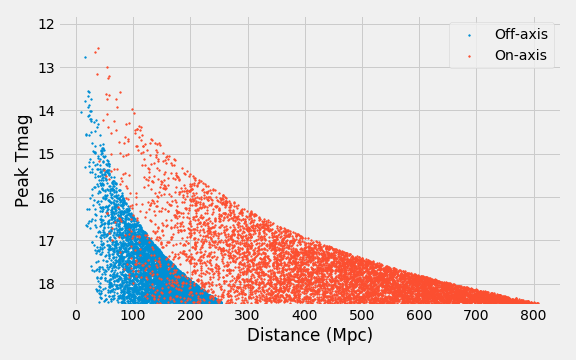
\includegraphics[width=0.8\textwidth]{events-per-centuary.png}
\caption{The range of distances and brightnesses of 100 years of events detectable by TESS. On-axis events are rare ($<$4\%) but are much more intrinsically bright. They can be detected as far out as 800 Mpc, while the off-axis events are typically within 250 Mpc. Most on-axis detections are too distant to be accompanied with a GW detection. Plotted are all events across the sky in a century that are detectable by TESS. With an instantaneous field-of-view of approximately 4.1\% of the sky, we anticipate 0.4--5 detections during the 2-year TESS primary mission, of which approximately 20\% will have an associated GW detection.}
\label{fig:event-distances}
\end{figure}

Although we can detect EM radiation from these events, not all will be detectable in gravitational waves. Firstly, LIGO/Virgo has a horizon, beyond which they are no longer sensitive. Secondly, while TESS will be observing near continuously, LIGO/Virgo shutdown for upgrades. During the 2018-2019 observing run of LIGO (O3), it is anticipated that the system will be sensitive to BNS mergers with sky and orientation averaged distances of 170 Mpc \citep{Abbott2016}, and will detect mergers up to 190 Mpc away once at design sensitivity in O4. We assume that for the 2-year TESS primary mission, LIGO (the larger, more sensitive interferometer) will be operational 60\% of the time, and will spend half of that time at the lower sensitivity of 170 Mpc and half at full sensitivity. We limited our sample by these and found final estimated detections of GW counterparts as $0.7^{+1.4}_{-0.5}$ during the 2-year TESS primary mission.

However, detection is not the same as characterization, and for TESS to be truly contribute scientifically we will need to capable of resolving structure in the light curve at early times. With a 5-$\sigma$ detection per 30-min integration, at peak brightness we have good resolving power of structure (c.f. Figure~\ref{fig:tesslc-distances}). For GW170817-like events, this means a peak brightness of Tmag$<$18.1. Including our model that integrates over the range of galaxy and BNS merger event brightnesses, limiting our yield to only those events that TESS will characterize the cuts our estimates slightly to 170$^{+180}_{-150}$ events per century. The number of events characterized during the TESS primary mission that will have simultaneous GW counterparts is slightly lower than the number of TESS detections at $0.6^{+1.2}_{-0.5}$.


\section{Discussion}
We are fortunate that such a bright, unambiguous kilonova detection was the first observed GW+EM event. However, it should be emphasized that we are extrapolating from a single event and that event may not be characteristic of the population. In our modeling in the previous section we have included ranges of peak brightness for kilonovae and GRB afterglows but we have assumed that all events follow the same spectral energy evolution. GW170817 was blue early and got fainter and redder over time. In some respects, this is a conservative assumption - if future events are redder than this at early times, then more light will fall into TESS' $\sim$0.6--1.0 bandpass. Let's now make an assumption that kilonova all have a peak wavelength of 0.8 $\mu$m ... [recalculate with different SED].


% ...\\
% talk about orphan events
% ...\\
% talk about detecting both afterglow and kilonova emission
% ...\\
% opening angle
% ...\\
% talk about choice of brightness prior, maybe also include a log-normal prior
% ...\\
We used an occurrence rate for BNS merger events of $1540^{+3200}_{-1220}$ Gpc$^{-3}$ yr$^{-1}$ that was derived by \citet{Abbott2017a} based on GW170817 and the LIGO/Virgo data alone. However, we could also use estimates from short-duration GRB (SGRB rates) or population synthesis models. These estimates have typically been significantly lower than found by \citet{Abbott2017a}. For example \citet{Fong2015} report a beaming corrected rate of $240^{+1580}_{-180}$ Gpc$^{-3}$ yr$^{-1}$ based on 11 SGRBs, while \citet{Chruslinska2017} use population synthesis models to predict a local rate of 48 Gpc$^{-3}$ yr$^{-1}$. We can use each of these estimates to revise our numbers. As expected, the detected yields decreases with the space density estimate used, declining to XX simultaneous TESS+GW detections during the primary mission if using the \citet{Fong2015} rate, and just 0.03 if using the \citet{Chruslinska2017} rate. Fortunately, we have reason to believe that the higher value is more reasonable. Firstly, that we observed an event that could have been seen by TESS makes it unlikely that the event rate could be as low as 48 Gpc$^{-3}$ yr$^{-1}$.



...\\
we should discuss PLATO, maybe WFIRST?? \textbf{Elisa} can help with WFIRST, maybe \textbf{Geert} can write something about PLATO. PLATO will observe 2250 deg2 per pointing but will go much deeper.

...\\
we could also comment on other transient phenomena. GRBs, certainly orphan afterglows, super novae? That way whenever someone wants to cite transients with tess they can use this paper. This is probably out of scope, but should be mentioned
...\\
say that TESS doesn't need VIRGO because it doesn't care about localization in the same way that ground-based efforts do.

\section{Conclusions}
With the announcement of GW170817, the era of multi-messenger astronomy has begun. The goal of this paper is to understand whether TESS can contribute to this field. We used flux-calibrated spectra collected with the Magellan telescopes that cover 0.49--8.46 days post-merger to estimate the brightness of this event in the TESS bandpass. Then, assuming a diversity of events based on models of GRB afterglow and kilonova models, we estimated the frequency of events that are bright enough for TESS to detect. The TESS mission-integrated average field of view if 4.1\% of they, therefore we predicted TESS might see \red{XX} events. However, LIGO/Virgo is not observing continually, and is not sensitive to events further away than $\sim$170--190 Mpc. We find that XX\% of events will not have a GW counterpart, and the total number of joint TESS+EM detections during the TESS 2-year primary mission will be XX events. 



\acknowledgments

The idea for this paper came while the lead author was sat watching the GW170817 press conference. We thank the LIGO and VIRGO teams, and the myriad space and ground-based observers for releasing the data so rapidly and with so much detailed analysis.


\software{Matplotlib \citep{matplotlib}, 
SciPy \citep{scipy},
NumPy \citep{numpy},
IPython \citep{ipython},
          }


% \begin{thebibliography}{}
% \end{thebibliography}

\bibliography{biblio}{}
\bibliographystyle{aasjournal}


\end{document}

% End of file `sample61.tex'.
